\documentclass{article}

\usepackage{algorithmic, amsmath, amsthm, amsfonts, amssymb,commath, enumerate, tikz, tikz-cd, color, mathrsfs} %tikz is for drawing lattices %tikz-cd is for commutative diagrams
															%color is for making notes in red 
															%mathrsfs is for power set font
%\usepackage[mathscr]{eucal} %mathscr gives nice script fonts

\newtheoremstyle{problemstyle}  % <name> This is my problemstyle. use begin{problem}.
        {12pt}                                               % <space above>
        {}                                               % <space below>
        {\itshape}                               % <body font>
        {}                                                  % <indent amount}
        {\bfseries}                 % <theorem head font>
        {\normalfont\bfseries.}         % <punctuation after theorem head>
        {.5em}                                          % <space after theorem head>
        {}                                                  % <theorem head spec (can be left empty, meaning `normal')>


\theoremstyle{problemstyle}

\newtheorem{problem}{Problem}

\theoremstyle{lemmastyle}

\newtheorem{lemma}{Lemma}

\theoremstyle{theoremstyle}

\newtheorem{theorem}{Theorem}

\title{ \vspace{-10ex} %uncomment to remove vertical space
%title of assignment goes here e.g. "Math 721 Homework 3"
An Algebraic Introduction to Mathematical Logic\\
Chapter 4 Predicate Calculus \\
Section 1 Algebra of Predicates \\
Proof of Transitivity 
}


\author{David L. Meretzky
}


\date{%date assignment is due goes here
May 30th, 2018
} 


\renewcommand*{\thefootnote}{$\dagger$} %changes default footnote marking to a dagger instead of a number (numbers are sometimes mistaken for citations)

\begin{document}

\maketitle

\begin{flushleft}
\textbf{Definition 1.3} Let $w \in \widetilde{P}(V,\mathscr{R})$ the $depth$ $of$ $quantification$ of $w$, denoted by $d(w)$, is defined by 

\begin{enumerate}
\item $d(\textbf{F}) = 0$, $d(r(x_1,x_2,...,x_n)) = 0$ for every free generator of $\widetilde{P}(V,\mathscr{R})$. Note, since $F_0$ in the construction of $\widetilde{P}(V,\mathscr{R})$ is the union of $T_0 = \{\textbf{F}\}$ and the generators which are of the form $r(x_1,x_2,...,x_n)$ for $r \in \mathscr{R}$ and $x_1,x_2,...,x_n \in V$, then we can say for all $f \in F_0$, $d(f) = 0$. 

\item $d(w_1 \Rightarrow w_2) = max(d(w_1),d(w_2))$

\item $d((\forall x)(w)) = 1 + d(w)$ for $x \in V$ 
\end{enumerate}
\end{flushleft}
Our desired congruence relation on $\widetilde{P}(V,\mathscr{R})$ may now be defined.

\begin{flushleft}
\textbf{Definition 1.4} Let $w_1$, $w_2 \in \widetilde{P}(V,\mathscr{R})$ define $w_1 \approx w_2$ if

\begin{enumerate}
\item $d(w_1) = d(w2) = 0$ and $w_1 = w_2$. 
%Generating the free proposition algebra on $F_0$ that is, all generators and $\textbf{F}$, that is $F_0$ are of depth 0. The use of $\Rightarrow$ does not increase the depth of quantification. Thus the equivalence relation on the proposition algebra contained in the predicate algebra $\widetilde{P}(V,\mathscr{R})$ is just equality. 
\item $d(w_1) = d(w_2) > 0$, $w_1 = a_1 \Rightarrow b_1$, $w_2 = a_2 \Rightarrow b_2$, $a_1 \approx a_2$ and $b_1 \approx b_2$ or 
\item $w_1 = (\forall x)(a)$, $w_2 = (\forall y)b$, and either
\begin{enumerate}
\item $x = y$ and $a \approx b$   
\item There exists a $c = c(x)$ such that $c(x) \approx a$ and $c(y) \approx b$ and $y \notin V(c)$ 
\end{enumerate}
\end{enumerate}
\end{flushleft}


\begin{problem}[Exercise 1.5 i)]
Given that $z \notin V(w_1) \cup V(w_2)$ show by induction over $d(w_1)$ that the element $c = c(x)$ in $\textbf{Definition 1.4}$ $3 (b)$ can always be chosen such that $z \notin V(c).$
\end{problem}

\begin{proof}
Assuming the notation of $\textbf{Definition 1.4}$ $3 (b)$, we have $c(x) \approx a$ and $c(y) \approx b$.\\ 

The base case $d(w_1) = 1$ holds because the relation $c(x) \approx a$ is equality for depth $0$ and therefore, $V(c(x)) = V(a)$. Since $w_1 = (\forall x)(a)$, we have that $z \notin V(a)$ and therefore, $z \notin V(c)$.\\ 

Now let $d(w_1) = n+1$. The relations $c(x) \approx a$ and $c(y) \approx b$ are happening at depth $n$. The claim is that at every depth $n$ the relations $c(x) \approx a$ and $c(y) \approx b$ can be replaced by depth $n-1$ expressions. Finally, since all expressions are finite compositions of operations, this process terminates at depth zero where we invoke the base case.\\ 

The relations $c(x) \approx a$ and $c(y) \approx b$ at depth $n > 0$ hold because of any one of the following 3 possiblilities: $\textbf{Definition 1.4}$ $2$, $\textbf{Definition 1.4}$ $3 (a)$ or $\textbf{Definition 1.4}$ $3 (b)$.  Note that $c(x) \approx a$ and $c(y) \approx b$ could each hold because of a different case potentially. However, their depths of quantification must match. 

So without loss of generality we just show how the relation $c(x) \approx a$ can be reduced to a lower depth expression  $\overline{c}(x) \approx \overline{a}$ while guaranteeing that $z \notin V(c) - V(\overline{c})$. 

\section*{Cases}
\subsection*{$\textbf{Definition 1.4}$ $\textbf{2}$} 
Assume now that $c(x) \approx a$ because of $\textbf{Definition 1.4}$ $2$. That is to say $a = a_1 \Rightarrow a_2$, $c = c_1 \Rightarrow c_2$, and therefore, $a_1 \approx c_1$ and $a_2 \approx c_2$. The definition of depth of $a$ is $max(a_1, a_2)$ and since  $a_1 \approx c_1$ and $a_2 \approx c_2$ implies that $d(a_1) = d(c_1)$ and $d(a_2) = d(c_2)$, $d(a) = d(max(a_1, a_2)) = d(max(c_1, c_2)) = d(c(x))$. We already knew in fact that $d(a) = d(c(x)$. Thus the relation $c(x) \approx a$ has been reduced to the two relations $a_1 \approx c_1$ and $a_2 \approx c_2$. One of these expressions is of depth equal to $c(x) \approx a$ and one is of depth less than or equal to $c(x) \approx a$.  The relations $a_1 \approx c_1$ and $a_2 \approx c_2$ each hold because of any one of the $3$ cases. Since (in prefix notation) an expression may only begin with at most finitely many $\Rightarrow$ eventually it will begin with a quantifier which brings us to cases 2 and 3 where we lower the depth of quantification in all cases. 

\subsection*{$\textbf{Definition 1.4}$ $\textbf{3 (a)}$} 
Assume now that $c(x) \approx a$ because of $\textbf{Definition 1.4}$ $3 (a)$. That is, $c(x) = \forall x_2\overline{c}(x_2,x)$ and $a(x) = \forall x_2\overline{a}(x_2,x)$. Then $\forall x_2\overline{c}(x_2,x) \approx \forall x_2\overline{a}(x_2,x)$ and $\overline{c}(x_2,x) \approx \overline{a}(x_2,x)$. The depth of the problem has just been reduced by one depth of quantification. Note that the relation $\overline{c}(x_2,x) \approx \overline{a}(x_2,x)$ could hold because of any one of the three cases. 

\subsection*{$\textbf{Definition 1.4}$ $\textbf{3 (b)}$} 
Assume now that $c(x) \approx a$ because there exists some $e(x_1)$ such that $e(x_1) \approx \overline{a}(x_1)$ and $e(x_2) \approx \overline{c}(x_2)$ where $a(x) = \forall x_1 \overline{a}(x_1,x)$ and $c(x) = \forall x_2 \overline{c}(x_2,x)$ and $x_2 \notin V(e(x_1))$. Now pick any variable $z' \notin V(w_1) \cup V(w_2)\cup V(c(x))$.  

By the induction hypothesis, $e(x_1)$ can be chosen so that it does not contain the variable $z'$. Thus we can substitute any mentions of the variable $z$ in $e(x_1)$ with $z'$ which we have ensured is not already present without disrupting the equivalence $c(x) \approx a$.  

Suppose however, that the variable $x_2 = z$, then we may rechose $x_2$ which is quantified over when it appears in $c(x)$ and $c(y)$. That is, $c(x) = \forall x_2c(x_2,x)$ so let $c'(x) = \forall x\overline{c}(x_3,x)$. The important thing is that $c'$ still works in $\textbf{Definition 1.4}$ $3 (b)$ for $w_1 \approx w_2$. By construction, it remains true that $a \approx c'(x)$ and $b \approx c'(y)$ because $e(x_1, x) \approx \overline{a}(x_1, x)$ and $e(x_3,x) \approx \overline{c}(x_3,x)$. $\textit{In the figure below both of the relations}$ $c(x) \approx a$ $\textit{and}$ $c(y) \approx b$ $\textit{hold because of case 3 although this need not be the case}$

%%% FIG 0 %%%%%
\begin{flushleft}
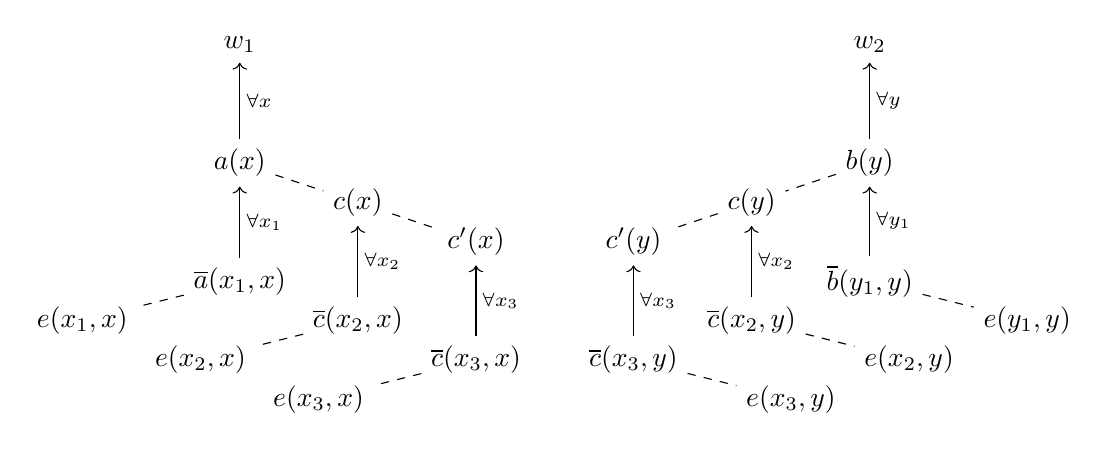
\begin{tikzpicture}[commutative diagrams/every diagram]
%\draw [help lines] (0,0) grid (12,4.5);
\node (P0) at (2,4.5) {$w_1$};
\node (P1) at (2,3) {$a(x)$};
\node (P2) at (2,1.5) {$\overline{a}(x_1,x)$};
\node (P3) at (10,4.5) {$w_2$};


\node (P4) at (10,3) {$b(y)$};
\node (P5) at (10,1.5) {$\overline{b}(y_1,y)$};
\node (P6) at (3.5,2.5) {$c(x)$};
\node (P7) at (8.5,2.5) {$c(y)$};

\node (P8) at (3.5,1) {$\overline{c}(x_2,x)$};
\node (P9) at (8.5,1) {$\overline{c}(x_2,y)$};

\node (P10) at (5,2) {$c'(x)$};
\node (P11) at (7,2) {$c'(y)$};

\node (P12) at (5,.5) {$\overline{c}(x_3,x)$};
\node (P13) at (7,.5) {$\overline{c}(x_3,y)$};

% es
\node (P14) at (0,1) {$e(x_1,x)$};
\node (P15) at (1.5,.5) {$e(x_2,x)$};
\node (P16) at (3,0) {$e(x_3,x)$};

\node (P17) at (12,1) {$e(y_1,y)$};
\node (P18) at (10.5,.5) {$e(x_2,y)$};
\node (P19) at (9,0) {$e(x_3,y)$};

\path[commutative diagrams/.cd, every arrow, every label]

%w_1 to a(x)
(P1) edge node[swap] {$\forall x$} (P0)

% \overline{a}(x_1, x) to a(x) 
(P2) edge node[swap] {$\forall x_1$} (P1)

%w_2 to b(y)
(P4) edge node[swap] {$\forall y$} (P3)

% \overline{b}(y_1, y) to a(y) 
(P5) edge node[swap] {$\forall y_1$} (P4)


%\overline{c}(x_2, x) to c(x)
(P8) edge node[swap] {$\forall x_2$} (P6)

% \overline{c}(y_1, y) to c(y) 
(P9) edge node[swap] {$\forall x_2$} (P7)

% similarity from a to c(y)
(P1) edge [-,dashed] (P6)

% similarity from b to c(y)
(P4) edge [-, dashed] (P7)

% similarity from a to c(y)
(P6) edge [-,dashed] (P10)

% similarity from b to c(y)
(P7) edge [-, dashed] (P11)

% similarity from a to c(y)
(P12) edge node[swap] {$\forall x_3$} (P10)

% similarity from a to c(y)
(P13) edge node[swap] {$\forall x_3$} (P11)


% eees
(P2) edge [-, dashed] (P14)
(P8) edge [-, dashed] (P15)
(P12) edge [-, dashed] (P16)

(P5) edge [-, dashed] (P17)
(P9) edge [-, dashed] (P18)
(P13) edge [-, dashed] (P19);

\end{tikzpicture}
\end{flushleft}

Therefore, $z \notin V(e(x_3))$, moreover, $z \neq x_3$.  In order to show that $z \notin c'(x)$ all that remains is to show that $z\notin V(\overline{c}(x_3)) - {x_3}$. Notice that we have just reduced the problem by one degree of quantification. 

More precisely, $z \notin V(e(x_3,x))$ and $z \notin V(e(x_3,y))$. Also, $e(x_3,x) \approx \overline{c}(x_3,x)$ and $e(x_3,y) \approx \overline{c}(x_3,y)$.  At the previous level, $a(x)$ played the role of $e(x_3,x)$ in the induction and $b(y)$ played the role of $e(x_3,y)$. Explicitly in the statement of the problem, since $x_3 \neq z$, we could let  $\forall x_3e(x_3,x)$ play the role of $w_1$ and depending on why $c(y) \approx b$ in case 3 let $\forall x_3e(x_3,y)$ play the role of $w_2$ or if $c(y) \approx b$ holds because of case $2$ let $b$ play the role of $w_2$, $c$ is then played by $\overline{c}(x_3,x)$. 

Thus we have reduced the depth of quantification by $1$. 
\end{proof}

% Here is a note now on why I believe it suffices to consider only the case where $a(x)$ and $b(x)$, and their lower depth analogues begin with a quantifier and not an $\Rightarrow$ operator. This is equivalent to saying that, $a(x) \approx c(x)$ and $b(y) \approx c(y)$ because of $\textbf{Definition 1.4}$ $3 (b)$. \\ 
% 
% From the definitions, in this case  $p_1 \approx p_2$   means that $(a_1 \Rightarrow b_1) \approx (a_2 => b_2)$  which happens iff $a_1 \approx a_2$ and $b_1 \approx b_2$.  However, the depth of the expression $d(p_j) = max(d(a_j),d(b_j))$. 
% 
% Taken together, this means that in $p_1 \approx p_2$, if $p_j$ begins with an implication $=>$, then this reduces to the case $a_1 \approx a_2$ if $d(a_1)>d(b_1)$ otherwise $b_1 \approx b_2$. Again, we always have $d(a_1) = d(a_2)$ if $a_1 \approx a_2$. By the maximality condition, $d(p_j) = d(a_j)$ and $d(a_j)$ begins with a quantifier (actually it just begins with one less implication but iterating this process we can remove all implications without affecting the depth of quantification).


% \begin{lemma}
% Assume that $a(x) \approx c(x)$. Then any variable in $V(c(x))$ not present in $V(a(x))$ may be rechosen arbitrarily from the infinite set of variables not present in either.  We show this by induction on the depth of quantification of $a(x)$.
% \end{lemma}
% 
% \begin{proof}
% Let $d(a(x)) = 0$. Then $a(x) = c(x)$ and therefore $V(c(x))\backslash V(a(x)) = \emptyset$. So the induction hypothesis holds in the base case.\\ 
% 
% Assume for all depths of quantification less than $n$ the induction hypothesis holds. Let $d(a(x)) = d(c(x)) = n$ and $a(x) \approx c(x)$. Also let $a(x) = \forall x_1 a_1(x,x_1)$ and $c(x) = \forall x_2 c_1(x,x_2)$. Then by $\textbf{Definition 1.4}$ $3 (b)$, there exists a $e(x,x_1)$ not containing $x_2$ such that $e(x,x_1) \approx a_1(x,x_1)$ and  $e(x,x_2) \approx c_1(x,x_2)$.\\
% 
% Since  the depth $d(a_1(x,x_1)) = d(e(x,x_1)) = n-1$ we have that any varible $z \in V(e(x,x_1))$ which is not in $a_1(x,x_1)$ can be rechosen arbitrarily. Since $e(x,x_2) \approx c_1(x,x_2)$, any variable $z \in V(c_1(x,x_2))$ not in $V(e(x,x_2))$ may be rechosen arbitrarily. I then claim that all variables of $V(c_1(x,x_2))$ not in $V(a_1(x,x_1))$. 
% 
% % may be rechosen arbitrarily, with the possible exception of $x_2$.\\  
% % 
% % By unfolding $e(x,x_1)$ and $e(x,x_2)$ one depth of quantification further and setting both congruent to themselves, we obtain $e(x,x_1) \approx e(x,x_2)$. Hence $x_2$ may be rechosen arbitrarily since $x_2 \notin V(e(x,x_1))$.\\
% 
% Suppose there is a variable $z \notin V(a_1(x,x_1))$ but present in $V(c_1(x,x_2))$.\\\\ Case 1. If $z \notin V(e(x,x_2))$, we can use the congruence $e(x,x_2) \approx c_1(x,x_2)$ to eradicate $z$.\\\\  Case 2. If $z \in V(e(x,x_2))$, then we can use the congruence $a_1(x,x_1) \approx e(x,x_1)$ to rechose $z$ in $e(x,x_1)$ if it appears there.  Consequently, the only place that $z$ could be in $e(x,x_2)$ is as in $x_2$, that is $z = x_2$.  this violates the assumption that y NEQ. 
% 
% It follows that any variable in $V(c_1(x,x_2))$ not present in $V(a_1(x,x_1))$ may be rechosen arbitrarily.
% 
% Since $a(x) = \forall x_1 a_1(x,x_1)$ and $c(x) = \forall x_2 c_1(x,x_2)$. The result follows: 
% \end{proof}
% 
% \begin{problem}[Exercise 1.5 i)]
% Given that $z \notin V(w_1) \cup V(w_2)$ show by induction over $d(w_1)$ that the element $c = c(x)$ in $\textbf{Definition 1.4}$ $3 (b)$ can always be chosen such that $z \notin V(c).$
% \end{problem}
% 
% \begin{proof}
% By definition, there exists a $c(x)$ as in $\textbf{Definition 1.4}$ $3 (b)$ such that if $w_1 = \forall x a_1(x)$ and $w_2 = \forall y a_2(y)$, we have $a_1(x) \approx c(x)$, $y \notin V(c(x))$, and $a_2(y) \approx c(y)$. 
% 
% By the lemma, since $a_1(x) \approx c(x)$, if $z \notin V(a(x))$, then if $z \in V(c(x))$, $z$ can be rechosen arbitrarily. Since $z \notin V(w_2)$, $z \neq y$. 
% \end{proof}

\begin{problem}[Exercise 1.5 ii)]
If $u(x) \approx v(x)$ and $y \notin V(u(x)) \cup V(v(x))$, show by induction over $d(u(x))$ that $u(y) \approx v(y)$.
\end{problem}

\begin{proof}
The base case holds because the relation is equality for depth $0$. 

Suppose the result holds for depth of quantification less than $n$. Then let $d(u(x)) = d(v(x)) = n$.  Let $u(x) = \forall x_1 u_1(x,x_1)$ and $v(x) = \forall x_2 v_1(x,x_2)$. Then there exists a $c(x,x_1)$  such that $u_1(x,x_1) \approx c(x,x_1)$ and $c(x,x_2) \approx v_1(x,x_2)$ such that $x_2 \notin V(c)$. By $\textbf{Problem 1}$ we have that $y \notin V(c)$.\\

By the induction hypothesis, since the depth of $u_1$ $v_1$ and $c$ are all $n-1$ we have that $u_1(y,x_1) \approx c(y,x_1)$ and $c(y,x_2) \approx v_1(y,x_2)$. Then by definition, since $u(y) = \forall x_1 u_1(y,x_1)$ and $v(y) = \forall x_2 v_1(y,x_2)$, we have proven $u(y) \approx v(y)$.
\end{proof}

\begin{problem}[Exercise 1.5 iii)]
Show that the relation is transitive. 
\end{problem}

\begin{proof}
Let $w_1 \approx w_2$ and $w_2 \approx w_3$. Assume the relation is transitive for lower depths of quantification. Since the relation is defined to be strict equivalence at depth $0$, the base case holds.\\\\ The proof is given in the worst possible case: We begin by twice invoking $\textbf{Definition 1.4}$ $3 (b)$. \\

Let $w_1 = \forall x a_1(x)$, $w_2 = \forall y a_2(y)$, and $w_3 = \forall z a_3(z)$. We have that there exists $c_1(x)$ and $c_2(y)$, such that $y \notin c_1(x)$ and $z \notin c_2(y)$. Also, because of $\textbf{Problem 1}$ we may require that $z \notin c_1(x)$ and $x \notin c_2(y)$.  By part $3 (b)$, of the definition $w_1 \approx w_2$ is defined to mean, $a_1(x) \approx c_1(x)$ and $c_1(y) \approx a_2(y)$. Likewise, $w_2 \approx w_3$ means that $a_2(y) \approx c_2(y)$ and $c_2(z) \approx a_3(z)$.\\

By the induction hypothesis, since $c_1(y) \approx a_2(y)$ and $a_2(y) \approx c_2(y)$, we have $c_1(y) \approx c_2(y)$. Note also that neither $c_1(y)$ nor $c_2(y)$ contains either $x$ or $z$.\\

By $\textbf{Problem 2}$ we have that  $c_1(x) \approx c_2(x)$. Then applying the induction hypothesis again, we obtain from $a_1(x) \approx c_1(x)$ and $c_1(x) \approx c_2(x)$, that $a_1(x) \approx c_2(x)$. Note also that since $c_2(z) \approx a_3(z)$, we have bridged the gap and it follows that $w_1 \approx w_3$.

Other cases follow from just $\textbf{Problem 1}$ and the induction hypothesis alone. 

\end{proof}

\end{document}